

\Chapter{Variant's generation}{RQ1. To what extent it is possible to artificially create variants for WebAssembly programs?} 
\label{chapter:generation}

% Define some numbers here for the autmation of the tables
\newcommand{\libsodiumfunctions}{687}
\newcommand{\qrcodefunctions}{1840}

\newcommand{\diversifiedsodium}{89}
\newcommand{\diversifiedqrcode}{130}
\newcommand{\libpopulation}{2408}
\newcommand{\qrpopulation}{4155}

% Execute a python script for small calculations
\newcommand{\py}[1]{\input{|python3 interpreter.py #1}}

\newcommand{\allmewefunctions}{\libsodiumfunctions + \qrcodefunctions}
\newcommand{\allmewediversified}{\diversifiedsodium + \diversifiedqrcode}
\newcommand{\allmewepopulation}{\libpopulation + \qrpopulation}



This chapter investigates whether we can artificially create program variants through semantically equivalent code transformations. We propose a framework to generate program variants functionally equivalent to their original.
We introduce the retargeting of a superoptimizer, using its exhaustive search strategy to provide semantically equivalent code transformations. 
The presented methodology and transformation tool, CROW, are contributions to this thesis.
We evaluate the usage of CROW on two corpora of open-source and nature diverse programs. 



\section{CROW}
\label{section:crow}
This section describes CROW, a tool tailored to create semantically equivalent variants out of a single program, either C/C++ code or LLVM bitcode. We assume that the \wasm programs are generated through the LLVM compilation pipeline to implement CROW. This assumption is supported by the work of Lehman et al. \cite{}; the fact that LLVM-based compilers are the most popular compilers to build \wasm programs \cite{usenixWASM2020} and the availability of source code (typically C/C++; and LLVM for \wasm) that provides a structure to perform code analysis and produce code replacements that is richer than the binary code. CROW is part of the contributions of this thesis.
In \autoref{diagrams:crow}, we describe the workflow of CROW to create program variants.

\begin{figure*}[h]
    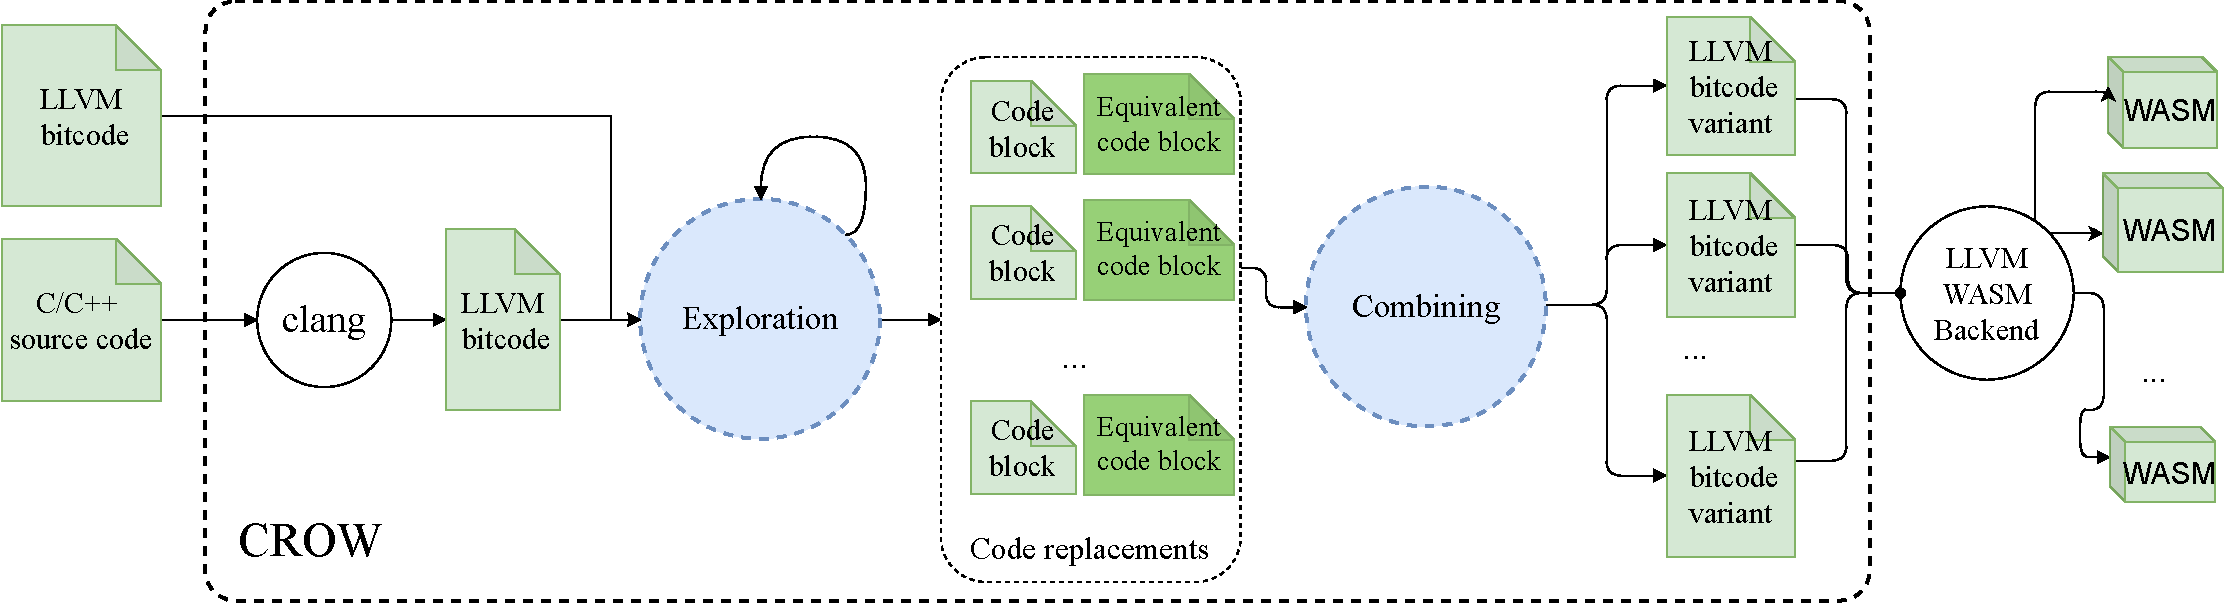
\includegraphics[width=\linewidth]{diagrams/generation/crow.drawio.pdf}
    \caption{CROW workflow to generate program variants. CROW takes C/C++ source codes or LLVM bitcodes to look for code blocks that can be replaced by semantically equivalent code and generates program variants by combining them.}
    \label{diagrams:crow}
\end{figure*}

Figure \ref{diagrams:crow} highlights the main two stages of the CROW's workflow, \textit{exploration} and \textit{combining}. The workflow starts by compiling the input program into the LLVM bitcode using clang from the source code. During the \emph{exploration} stage, CROW takes an LLVM bitcode and, for its code blocks, produces a collection of code replacements that are functionally equivalent to the original program. In the following, we enunciate the definitions we use along with this work for a code block, functional equivalence, and code replacement. 


\begin{definition}{Block (based on Aho \etal \cite{10.5555/6448}):}\label{def:code-block}
    Let $P$ be a program. A block $B$ is a grouping of declarations and statements in $P$ inside a function $F$. 
\end{definition}


\begin{definition}{Functional equivalence modulo program state (based on Le \etal \cite{10.1145/2594291.2594334}):}
    \label{def:functional-equivalence}
    Let $B_1$ and $B_2$ be two code blocks according to \autoref{def:code-block}. We consider the program state before the execution of the block, $S_i$, as the input and the program state after the execution of the block, $S_o$, as the output. $B_1$ and $B_2$ are functionally equivalent if given the same input $S_i$ both codes produce the same output $S_o$.
\end{definition}

\begin{definition}{Code replacement:}
    \label{def:code-replacement}
    Let $P$ be a program and $T$ a pair of code blocks $(B_1, B_2)$. $T$ is a candidate code replacement if $B_1$ and $B_2$ are both functionally equivalent as defined in \autoref{def:functional-equivalence}.
    Applying $T$ to $P$ means replacing $B_1$ by $B_2$. The application of $T$ to $P$ produces a program variant $P'$ which consequently is functionally equivalent to $P$.     
\end{definition}

We implement the \emph{exploration} stage by retargeting a superoptimizer for  LLVM, using its subset of the LLVM intermediate representation. CROW operates at the code block level, taking them from the functions defined inside the input LLVM bitcode module. In addition, the retargeted superoptimizer is in charge of finding the potential places in the original code blocks where a replacement can be applied. Finally, we use the enumerative synthesis strategy of the retargeted superoptimizer to generate code replacements.
The code replacements generated through synthesis are verified, according to \autoref{def:functional-equivalence}, by internally using a theorem prover. 

Moreover, we prevent the superoptimizer from synthesizing instructions that have no correspondence in \wasm for the sake of reducing the searching space for equivalent program variants. Besides, we disable all optimizations in the \wasm LLVM backend that could reverse the superoptimizer transformations, such as constant folding and instructions normalization.

%\todo{We disable cost restrictions and the LLVM backend optimizations...maybe for the assesment RQ ?}

In the \emph{combining} stage, CROW combines the candidate code replacements to generate different LLVM bitcode variants, selecting and merging the code replacements. 
Then for each combination, a variant bitcode is compiled into a \wasm binary if requested. Finally, CROW generates the variants from all possible combinations of code replacements as the power set of all code replacements.  

\subsection{Example}
\label{section:crow:example}
 Let us illustrate how CROW works with the simple example code in \autoref{CExample}. The \texttt{f} function calculates the value of $2 * x + x$ where \texttt{x} is the input for the function.  CROW compiles this source code and generates the intermediate LLVM bitcode in the left most part of \autoref{example:crow:original:llvm}. CROW potentially finds two code blocks to look for variants, as the right-most part of \autoref{example:crow:original:llvm} shows.

% snippet of code showing the detection of code blocks
    
\begin{code}
    \lstset{language=C,
    basicstyle=\small\ttfamily,caption={C function that calculates the quantity $2x + x$},label=CExample}
    \begin{lstlisting}[style=CStyle]
int f(int x) { 
    return 2 * x + x; 
}    
    \end{lstlisting}
    
\end{code}

\lstdefinelanguage{LLVM}
    {morekeywords={i32,mul,align,nsw,add,load,store,define,br, ret, shl, ret},
    sensitive=false,
    morecomment=[l]{;},
    morecomment=[s]{;}{;},
    morestring=[b],
}
\lstdefinestyle{nccode}{
    numbers=left,
    tabsize=4,
    showspaces=false,
    breaklines=true, 
    showstringspaces=false,
    moredelim=**[is][{\btHL[fill=black!10]}]{`}{`},
    moredelim=**[is][{\btHL[fill=celadon!40]}]{!}{!}
}
\lstset{
    language=LLVM,
    style=nccode,
    %basicstyle=\small\ttfamily,
    columns=fullflexible,
    breaklines=true
}


\begin{code}
    \centering
    \captionof{lstlisting}{LLVM's intermediate representation program, its extracted instructions and replacement candidates. Gray highlighted lines represent original code, green for code replacements. }\label{example:crow:original:llvm}
    \lstset{numbers=none}
    \noindent\begin{minipage}[t]{.33\linewidth}
    \centering
    \begin{lstlisting}[xleftmargin=1em,escapechar=?]
    define i32 @f(i32) {

    ?\tikzmarkWS{2}{code 2}{11.5}{10}{3.5cm}?
    ?\tikzmarkWS{1}{code 1}{11.5}{3.5}{3.0cm}?
    %2 = mul nsw i32 %0,2
    %3 = add nsw i32 %0,%2 

    ret i32 %3
    }
    
    define i32 @main() {
    %1 = tail call i32 @f(i32 10)
    ret i32 %1
    }
    \end{lstlisting}
    \end{minipage}%\hfill%
    \begin{minipage}[t]{.32\linewidth}
        \begin{lstlisting}[xleftmargin=1em,escapechar=?]
?Replacement candidates for code\_1?

`%2 = mul nsw i32 %0,2`

!%2 = add nsw i32 %0,%0!

!%2 = shl nsw i32 %0, 1:i32!
    \end{lstlisting}
    \end{minipage}%\hfill%
    \begin{minipage}[t]{.32\linewidth}
        \lstdefinestyle{nccode}{
        tabsize=4, 
        showspaces=false,
        breaklines=true, 
        showstringspaces=false,
        moredelim=**[is][{\btHL[fill=black!10]}]{`}{`},
        moredelim=**[is][{\btHL[fill=celadon!40]}]{!}{!}
        }
        \lstset{
            language=LLVM,
            style=nccode,
            columns=fullflexible,
            breaklines=true,
            belowcaptionskip=1pt,
            abovecaptionskip=1pt,
        } 
        \begin{lstlisting}[name={B},escapechar=?]
?Replacement candidates for code\_2?

`%3 = add nsw i32 %0,%2`

!%3 = mul nsw %0, 3:i32!
        \end{lstlisting}
    \end{minipage}
    
\end{code}





\begin{code}
    \centering
    \captionof{lstlisting}{Candidate code replacements combination. Orange highlighted code illustrate replacement candidate overlapping.}\label{example:crow:original:combination}
    \lstset{numbers=none}
    \noindent\begin{minipage}[t]{.5\linewidth}
    \begin{lstlisting}[xleftmargin=1em,escapechar=?]
`%2 = mul nsw i32 %0,2`
`%3 = add nsw i32 %0,%2`

!%2 = add nsw i32 %0,%0!
`%3 = add nsw i32 %0,%2`

!%2 = shl nsw i32 %0, 1:i32!
`%3 = add nsw i32 %0,%2`

    \end{lstlisting}
    \end{minipage}%\hfill%
    \begin{minipage}[t]{.5\linewidth}
        \lstdefinestyle{nccode}{
        tabsize=4, 
        showspaces=false,
        breaklines=true, 
        showstringspaces=false,
        moredelim=**[is][{\btHL[fill=black!10]}]{`}{`},
        moredelim=**[is][{\btHL[fill=celadon!40]}]{!}{!},
        moredelim=**[is][{\btHL[fill=weborange!40]}]{'}{'}
        }
        \lstset{
            language=LLVM,
            style=nccode,
            columns=fullflexible,
            breaklines=true,
            belowcaptionskip=1pt,
            abovecaptionskip=1pt,
        } 
        \begin{lstlisting}[xleftmargin=1em,escapechar=?]
'%2 = mul nsw i32 %0,2'
!%3 = mul nsw %0, 3:i32!

'%2 = add nsw i32 %0,%0'
!%3 = mul nsw %0, 3:i32!

'%2 = shl nsw i32 %0, 1:i32'
!%3 = mul nsw %0, 3:i32!

    \end{lstlisting}
    \end{minipage}
\end{code}


\begin{tikzpicture}[remember picture,overlay]
%\path (2.north) edge[<-, bend left] (1.north);
%\path[draw, ->] (3.west) edge[<-, bend left] (2.west);
%\path (4.west) edge[<-, bend left] (3.west);
%\path (1.south) edge[<-, bend left] (4.south);

%\path (2.east) edge[<-, bend left, blue] (5.north);
%\path (3.east) edge[<-, bend right, olive] (2.east);
%\path (1.east) edge[<-, bend left, black] (replall1.west);
%\path (2.east) edge[<-, bend left, black] (replall2.west);
%\path (rep11.east) edge[<-, bend left, black] (6.east);
%\path (9.east) edge[<-, bend right, black] (4.east);
%\path (7.east) edge[<-, bend right, black] (8.east);
%\path (5.south) edge[<-, bend right, blue] (4.east);
%\path (9.north) edge[<-] (8.south);
%\path (5.south) edge[<-, bend left] (9.south);


%\path (10.north) edge[<-, bend left] (11.north);
%\path (11.south) edge[<-, bend left] (10.south);
%\path (7) edge[<-, bend right] (6.east);
%\path (8) edge[<-, bend right] (7.east);
\end{tikzpicture}


    

CROW, in the exploration stage detects 2 code blocks, \texttt{code\_block\_1} and \texttt{code\_block\_2} as the enclosing boxes in the left most part of \autoref{example:crow:original:llvm} show. CROW synthesizes $2 + 1$ candidate code replacements for each code block respectively as the green highlighted lines show in the right most parts of \autoref{example:crow:original:llvm}.
The baseline strategy of CROW is to generate variants out of all possible combinations of the candidate code replacements, \ie uses the power set of all candidate code replacements.

In the example, the power set is the cartesian product of the found candidate code replacements for each code block, including the original ones, as \autoref{example:crow:original:combination} shows. The power set size results in $6$ potential function variants. Yet, the generation stage would eventually generate $4$ variants from the original program. CROW generated 4 statically different Wasm files, as \autoref{example:crow:variants:wasm} illustrates. This gap between the potential and the actual number of variants is a consequence of the redundancy among the bitcode variants when composed into one. In other words, if the replaced code removes other code blocks, all possible combinations having it will be in the end the same program. In the example case, replacing \texttt{code\_block\_2} by \texttt{mul nsw \%0, 3}, turns \texttt{code\_block\_1} into dead code, thus, later replacements generate the same program variants. The rightmost part of \autoref{example:crow:original:combination} illustrates how for three different combinations, CROW produces the same variant. We call this phenomenon an overlapping.

One might think that a reasonable heuristic could be implemented to avoid such overlapping cases. Instead, we have found it easier and faster to generate the variants with the combination of the replacement and check their uniqueness after the program variant is compiled. This prevents us from having an expensive checking for overlapping inside the CROW code. Still, this phenomenon calls for later optimizations in future works.

\lstdefinestyle{nccode}{
        numbers=none,
        firstnumber=2,
        stepnumber=1,
        numbersep=10pt,
        tabsize=4, 
        showspaces=false,
        breaklines=true, 
        showstringspaces=false,
    moredelim=**[is][\btHL]{`}{`},
    moredelim=**[is][{\btHL[fill=black!10]}]{`}{`},
    moredelim=**[is][{\btHL[fill=celadon!40]}]{!}{!}
}

\lstset{
    language=WAT,
    style=nccode,
    basicstyle=\footnotesize\ttfamily,
    columns=fullflexible,
    breaklines=true
}


\begin{code}
    \centering
    \captionof{lstlisting}{\termidx{Wasm }program variants generated from program \autoref{CExample}.}\label{example:crow:variants:wasm}
    \lstset{numbers=none}
    \noindent\begin{minipage}[t]{.45\linewidth}
    \begin{lstlisting}[xleftmargin=1em,escapechar=?]
func $f (param i32) (result i32)
   local.get 0
    `i32.const 2`
    `i32.mul`
    `local.get 0`
    `i32.add`

        \end{lstlisting}
\begin{lstlisting}[xleftmargin=1em,escapechar=?]
func $f (param i32) (result i32)
    local.get 0
    !local.get 0!
    !i32.add!
    `local.get 0`
    `i32.add`

                \end{lstlisting}
    \end{minipage}\hfill
    \noindent\begin{minipage}[t]{.45\linewidth}
\begin{lstlisting}[xleftmargin=1em,escapechar=?]
func $f (param i32) (result i32)
    local.get 0
    !i32.const 1!
    !i32.shl!
    `local.get 0`
    `i32.add`

    \end{lstlisting}
\begin{lstlisting}[xleftmargin=1em,escapechar=?]
func $f (param i32) (result i32)
    local.get 0
    !i32.const 3!
    !i32.mul!

            \end{lstlisting}
        \end{minipage}
\end{code}





\section{Evaluation}
\label{section:crow:exp_setup}

We use CROW, the tool described at \autoref{section:crow}, to answer RQ1. This section describes the corpora of original programs that we pass to CROW for the sake of variants generation. Besides, we describe our metrics and finalize the section by discussing the results.

\subsection{Corpora}
\label{section:crow:corpora}

We answer RQ1 with two corpora of programs appropriate for our experiments. The first corpus, \textbf{CROW prime}, is part of the CROW contribution \cite{}. The second corpus, \textbf{MEWE prime}, is part of the MEWE contribution \cite{}. In \autoref{table:corpora} we summarize the selection criteria, and we mention each corpus properties. With both corpora we evaluate CROW with a total of $303 + \py{\allmewefunctions}$ functions. 

\subsection{Metric}
 
To assess our approach's ability to generate \wasm binaries that are statically different, we compute the number of unique variants generated by CROW for each original function. 
We compare the \wasm program and its variant using the \texttt{md5} hash of each function byte stream as a metric for uniqueness.


\begin{table}[h]
    \renewcommand{\arraystretch}{1.5}
    \footnotesize
    \centering
    \begin{tabular}{p{1cm} p{6cm} p{5cm}}
        Corpus name & Selection criteria & Corpus Description \\
        \midrule
        \textbf{CROW prime} & We take programs from the  Rosetta Code project\footnote{\url{http://www.rosettacode.org/wiki/Rosetta_Code}}. 
        %This website hosts a curated set of solutions for specific programming tasks in various  programming languages.
        %It contains a wide range of tasks, from simple ones, such as adding two numbers, to complex algorithms like a compiler lexer. 
        We first collect all C programs from Rosetta Code, which represents $989$ programs as of 01/26/2020. 
        
        We then apply a number of filters: the programs should successfully compile, they should not require user inputs, the programs should terminate and should not provide in non-deterministic results.  
        The result of the filtering is a corpus of 303 C programs  &  All programs have a single function in terms of source code. These programs range from $7$ to $150$ lines of code and solve a variety of problems, from the \textit{Babbage} problem to  \textit{Convex Hull} calculation. \\
        \hline
        \textbf{MEWE prime} & We select two mature and typical edge-cloud computing projects for this corpus.
        The projects are selected based on their suitability for  diversity synthesis with CROW, \ie the projects should have the ability to collect their modules in LLVM intermediate representation
        
        %, suitability for deployment on the Fastly infrastructure (the project should be easily portable Wasm/WASI and compatible with the Rust Fastly API). 

        The selected projects are: \textbf{libsodium}, an encryption, decryption, signature and password hashing library which can be ported to WebAssembly and \textbf{qrcode-rust}, a QrCode and MicroQrCode generator written in Rust. 
        
        &  The evaluated projects contain in total \py{\allmewefunctions} functions, \libsodiumfunctions\ for libdosium and \qrcodefunctions\ for qrcode-rust. The functions range between 10 ad 127700 lines of code. \\
    \end{tabular}
    \caption{Corpora description. The table is composed by the name of the corpus, the selection criteria and the stats the programs in each corpus.}
    \label{table:corpora}
\end{table}

\todo{Move text out of the table}



\subsection{Setup}

CROW's workflow synthesizes program variants with an enumerative strategy. All possible programs that can be generated for a given language (LLVM in the case) are constructed and verified for equivalence.
There are two parameters to control the size of the search space and hence the time required to traverse it.
On the one hand, one can limit the size of the variants. On the other hand, one can limit the set of instructions used for the synthesis. On the other hand, in our experiments, we use between $1$ instruction (only additions) and $60$ instructions (all supported instructions in the synthesizer).


These two configuration parameters allow the user to find a trade-off between the number of variants that are synthesized and the time taken to produce them. In \autoref{table:corpora:setup} we listed the configuration for both corpora. For the current evaluation, given the size of the corpus, we set the exploration time to 1 hour maximum per function for \textbf{CROW PRIME}. In the case of \textbf{MEWE prime}, we set the timeout to 5 minutes per function in the exploration stage. We set all 60 supported instructions in CROW for both \textbf{CROW prime} and \textbf{MEWE primer} corpora.

\begin{table}[H]
    \renewcommand{\arraystretch}{1.2}
    \centering
    \begin{tabular}{l | l l}
        \midrule
        CORPUS & Exploration timeout & Max. instructions \\
        \hline
        CROW prime & 1h & 60 \\
        MEWE prime & 5m & 60 \\
    \end{tabular}
    \caption{CROW tweaking for variants generation. The table is composed by the name of the corpus, the timeout parameter and the count of allowed instructions during the synthesis process.}
    \label{table:corpora:setup}
\end{table}

\section{Results}

We summarize the results in \autoref{table:crow:general_results}.
CROW produces at least one unique program variant for $239/303{}$ single function programs for \textbf{CROW prime} with 1h for timeout. For the rest of the programs ($64/303{}$), the timeout is reached before CROW can find any valid variant. 
In the case of \textbf{MEWE prime}, CROW produces variants for $\py{\allmewediversified}/\py{\allmewefunctions}$ functions with 5 minutes per function as timeout. The rest of the functions resulted in timeout before finding function variants or produce no variants.

{
    \renewcommand{\arraystretch}{1.6}
\begin{table}[h]
    \centering
    %\setlength\minrowclearance{1.0pt}
        \begin{tabular}[t]{ l  l  l  l  l }
            \midrule
        CORPUS & \#Functions & \# Diversified & \# NonDiversified & \# Variants  \\
        \hline   

        CROW prime & 303 & \textbf{239} & 64 & 1906    \\
        \hline
        MEWE prime & \pypy{\allmewefunctions} & \pypy{\allmewediversified} & \pypy{{\allmewefunctions} - {\allmewediversified}} & \textbf{\pypy{\allmewepopulation}}    \\
        \hline


        \end{tabular}
    
        \caption{General diversification results. The table is composed by the name of the corpus, the number of functions, the number of succesfully diversified functions, the number of non-diversified functions and the cumulative number of variants.}
        \label{table:crow:general_results}
\end{table}
}


\subsection{Challenges for automatic diversification}



CROW generates variants for functions in both corpora. However, we have observed a remarkable difference between the number of successfully diversified functions versus the number of failed-to-diversify functions, as it can be appreciated in \autoref{table:crow:general_results}. CROW successfully diversified approx. 79 \% and \py{100*{\allmewediversified} / {\allmewefunctions}}\% of the original functions for \textbf{CROW prime} and  \textbf{MEWE prime} respectively. On the other hand, CROW generated more variants for \textbf{MEWE prime}, \py{\allmewepopulation} program variants for \py{\allmewediversified} diversified programs. Not surprisingly, setting the timeout affects the capacity of CROW for diversification. On the other hand, a low timeout for exploration gives CROW more power to combine code replacements. This can be appreciated in the last column of the table, where for a lower number of diversified functions, CROW created, overall, more variants.



Moreover, we look at the cases that yield a few variants per function. There is no direct correlation between the number of identified codes for replacement and the number of unique variants. Therefore, we manually analyze programs that include many potential places for replacements, for which CROW generates few or no variants. 
We identify two main challenges for diversification.

\emph{1) Constant computation}  We have observed that Souper searches for a constant replacement for more than $45\%$ of the blocks of each function while constant values cannot be inferred. For instance,  constant values cannot be inferred for memory load operations because CROW is oblivious to a memory model. 

%\todo{Add example here}

% candidates overlapping
\emph{2) Combination computation}  The overlap between code blocks, mentioned in \autoref{section:crow:example}, is a second factor that limits the number of unique variants. CROW can generate a high number of variants, but not all replacement combinations are necessarily unique. 

%\todo{Add all the found examples here}


\subsection{Properties for large diversification using CROW}

We manually analyzed the programs that yield more than 100 unique variants to study the critical properties of programs leveraging a high number of variants.
This reveals one key reason that favors many unique variants: the programs include bounded loops. In these cases, CROW synthesizes variants for the loops by replacing them with a constant if the constant inferring is successful. Every time a loop constant is inferred, the loop body is replaced by a single instruction. This creates a new, statically different program. The number of variants grows exponentially if the function contains nested loops for which CROW can successfully infer. 

A second key factor for synthesizing many variants relates to the presence of arithmetic. Souper, the synthesis engine used by CROW, effectively replaces arithmetic instructions with equivalent instructions that lead to the same result. For example, CROW generates unique variants by replacing multiplications with additions or shift left instructions (\autoref{add:example}). Also, logical comparisons are replaced, inverting the operation and the operands (\autoref{cmp:examples}). Besides, CROW can use overflow and underflow of integers to produce variants (\autoref{overflow:example}), using the intrinsics of the underlying computation model.

{
\begin{code}
    \footnotesize
    \lstdefinestyle{nccode}{
        numbers=none,
        firstnumber=2,
        stepnumber=1,
        numbersep=10pt,
        tabsize=4, 
        showspaces=false,
        breaklines=true, 
        showstringspaces=false,
        moredelim=**[is][\btHL]{`}{`},
        moredelim=**[is][{\btHL[fill=black!10]}]{`}{`},
        moredelim=**[is][{\btHL[fill=celadon!40]}]{!}{!}
    }

    \lstset{
        language=WAT,
        style=nccode,
        basicstyle=\footnotesize\ttfamily,
        columns=fullflexible,
        breaklines=true
    }
    \noindent\begin{minipage}[b]{0.32\linewidth}
        \captionof{lstlisting}{Diversification through arithmetic expression replacement.}\label{add:example}
        \noindent\begin{minipage}[t]{0.46\linewidth}
            \begin{lstlisting}
local.get 0
`i32.const 2`
`i32.mul`
            \end{lstlisting}
        \end{minipage}%
        \hfill\noindent\begin{minipage}[t]{0.46\linewidth}
            
            \begin{lstlisting}
local.get 0
!i32.const 1!
!i32.shl!
            \end{lstlisting}
        \end{minipage}
    \end{minipage}\hfill%
    \begin{minipage}[b]{0.31\linewidth}
        \captionof{lstlisting}{Diversification through inversion of comparison operations.}\label{cmp:examples}
        \begin{minipage}[t]{.46\linewidth}
            \begin{lstlisting}
`local.get 0`
`i32.const 10`
`i32.gt_s`
            \end{lstlisting}
        \end{minipage}\hfill\begin{minipage}[t]{.46\linewidth}
           
            \begin{lstlisting}
!i32.const 11!
!local.get 0!
!i32.le_s!
            \end{lstlisting}
        \end{minipage}%
        
        
    \end{minipage}\hfill\noindent
    \noindent\begin{minipage}[b]{0.32\linewidth}
        \captionof{lstlisting}{Diversification through overflow of integer operands.}\label{overflow:example}
        \noindent\begin{minipage}[t]{0.46\linewidth}
            \begin{lstlisting}
`i32.const 2`
i32.mul
\end{lstlisting}
        \end{minipage}%
        \hfill\noindent\begin{minipage}[t]{0.46\linewidth}
            
            \begin{lstlisting}
i32.const 2
i32.mul
!i32.const -2147483647!
!i32.mul!
            \end{lstlisting}
        \end{minipage}
    \end{minipage}
    \end{code}
}

% \input{parts/example_rq1_replacements}



% \input{parts/example_rq1_babbage}


%We now discuss the prevalence of the transformations made by CROW when the \wasm binaries are transformed to machine code, specifically with the V8's engine. In \autoref{fig:rq1} we plot the cumulative distribution of
%\DTWStatic{}, comparing \wasm binaries (in blue) and x86 binaries (in orange). The figure plots  a total of 103003 \DTWStatic{} values for each representation, two values for each variant pair comparison (including original) for the 239 program.
%The value on the y-axis shows which percentage of the total comparisons lie below the corresponding \DTWStatic{} value on the x-axis.
%Since we measure the distances between original programs and \wasm variants, then $100\%$ of these  binaries have $\DTWStatic{}>0$.
%Let us consider the x86 variants: \DTWStatic{} is strictly positive for \nPreservedPercent{} of variants. In all these cases, the V8 compilation phase does not undo the CROW diversification transformations.
%Also, we see that there is a gap between both distributions, the main reason is the natural inflation of machine code. For example, two variants that differ by one single instruction in \wasm, can be translated to machine code where the difference is increased by more than one machine code instruction.

% Negative prevalence
%The zoomed subplot focuses on the beginning of the distribution, it shows that the \DTWStatic{} is zero for $0.52\%$ of the x86 binaries.
%In these cases the V8 TurboFan compiler from \wasm to x86 reverts the CROW transformations.
%We find that CROW produces at least one of these reversible transformations for $34/303Diversified{}$ programs.
%\autoref{add:prevalence_example} shows one of the most common transformations that is reversed by TurboFan, according to our experiments.

%Besides, local variables reordering and common subexpressions are cases that TurboFan reverses.
%\input{parts/non-prevalence-example}




\subsection{Variant properties}

Regarding the potential size overhead of the generated variants, we have compared the \wasm binary size of the diversified programs with their variants. The ratio of size change between the original program and the variants ranges from 82\% (variants are smaller) to 125\% (variants are larger) for \textbf{CROW prime} and \textbf{MEWE prime}. This limited impact on the binary size of the variants is good news because they are meant to save bandwidth when they become assets to distribute over the network.

\pagebreak
\section{Conclusions}

The proposed methodology can generate program variants that are syntactically different from their original versions. We have shown that CROW generates diversity among the binary code variants using semantically equivalent code transformations. We identified the properties that original programs should have to provide a handful number of variants. Besides, we enumerated the challenges faced to provide automatic diversification by retargeting a superoptimizer.

In the next chapter, we evaluate the assessment of the generated variants answering to what extent the artificial programs are different from the original in terms of static difference, execution behavior, and preservation.

\let\cleardoublepage\clearpage